\documentclass{article}


\title{Forschungsarbeit}
\author{Laura Schillke, Sebastian Meidel, Mekong Lam }
\date{October 2018}

% Pakete laden 
\usepackage[utf8]{inputenc}
\usepackage{graphicx}
\usepackage[german]{babel}
\usepackage[default,osfigures,scale=0.95]{opensans}  %% Option 'sfdefault' only if the base font of the document is to be sans serif
\usepackage[T1]{fontenc}
% Verlinke Zitate
\usepackage{hyperref}
% Verlinke das Inhaltsverzeichnis
\hypersetup{linktocpage}
\usepackage[style=footnote-dw, 
natbib=true, 
backref=true, 
edsuper=true, 
nopublisher=false, 
urldate=long, 
backend=biber]{biblatex}
\usepackage{csquotes}
\usepackage{graphicx}
\addbibresource{mendeley_v3.bib}


%Dokument beginnt
\begin{document}

\maketitle


\newpage

\setcounter{tocdepth}{3}
\tableofcontents 



\newpage

\section{Zusammenfassung}
Bacon ipsum dolor amet shank biltong t-bone ham, ground round pastrami boudin porchetta cow fatback turkey pork tenderloin salami. Buffalo meatloaf ham hock alcatra. Boudin ground round chicken porchetta ham. T-bone spare ribs chuck fatback.

\section{Einleitung}
Bacon ipsum dolor amet shank biltong t-bone ham, ground round pastrami boudin porchetta cow fatback turkey pork tenderloin salami. Buffalo meatloaf ham hock alcatra. Boudin ground round chicken porchetta ham. T-bone spare ribs chuck fatback.

%\begin{figure}[h!]
%\centering
%
\includegraphics[scale=1.7]{universe}
%\caption{The Universe}
%\label{fig:universe}
%\end{figure}

\section{Definitionen}

\subsection{Stadt}

Haas und Neumair zufolge bezeichnet man eine Stadt als eine größere verdichtete Siedlung, die mit bestimmten Funktionen und Merkmalen charakterisiert wird \cite{HaasDefinitionWirtschaftslexikon}. Die Brockhausdefinition schreibt einer Stadt Merkmale zu wie zum Beispiel die eigene Versorgungs- und Verwaltungsstruktur, die innere Gliederung oder eine höhere Bebauungs- und Verkehrsdichte. Hinzu kommen spezielle Funktionen wie poltische Aufgaben (Haupstädte, Festungsstädte) oder wirtschaftliche Funktionen (Hansestädte, Hafenstädte, Karawanenstädte) \cite{BrockhausStadt}. Die statistischen Kriterien, die eine „Stadt“ vom „Land“ unterscheiden variieren von Land zu Land. Beispielsweise werden Städte in der Bundesrepublik Deutschland mit 
\begin{itemize}
\item 5.000 bis 20.000 Einwohnern als „Kleinstadt“,
\item 20.000 bis 50.000 Einwohnern als „Mittelstadt“,
\item ab 100.000 Einwohnern als „Großstadt“ 
\end{itemize}
bezeichnet \cite{Institutinternationaldestatistique1887BulletinStatistique}. Demgegenüber orientiert man sich in China an die Bevölkerungsdichte: 

\begin{displayquote}
In the case of cities with district establishment, the city proper refers to the whole administrative area of the district if its population density is 1 500 people per kilometre or higher [...]. \cite[S.~2]{UnitedNations2005Table2005} 
\end{displayquote}

Unabhängig von regional unterschiedlichen Kriterien lässt sich mit steigender Einwohnerzahl und -dichte einer Stadt folgern, dass auch die Anforderung an gewährleisteter Infrastruktur und Lebensmittelversorgung für die städtische Bevölkerung steigt. D.h. die Lebensmittelversorgung einer Großstadt zu gewährleisten ist schwieriger als die einer Kleinstadt. Noch größer ist die Herausforderung in Megastädten. Den Vereinten Nationen zufolge wird eine Megastadt (englisch: „Megacity“) als eine Stadt bezeichnet mit mindestens 10 Millionen Einwohnern. Im Jahr 2016 existierten 31 Megastädte und Prognosen zufolge steige die Anzahl der Megastädte im Jahr 2030 auf 41 \cite{UnitedNations2016The2016}. Tokio zählt mit 38 Millionen Einwohnern als die größte Megastadt weltweit und derzeit befinden sich die meisten Megastädte in Industrie- und Entwicklungsländern (wie in Abbildung \ref{figUrban} erkennbar). 

\begin{figure}[h]
\centering
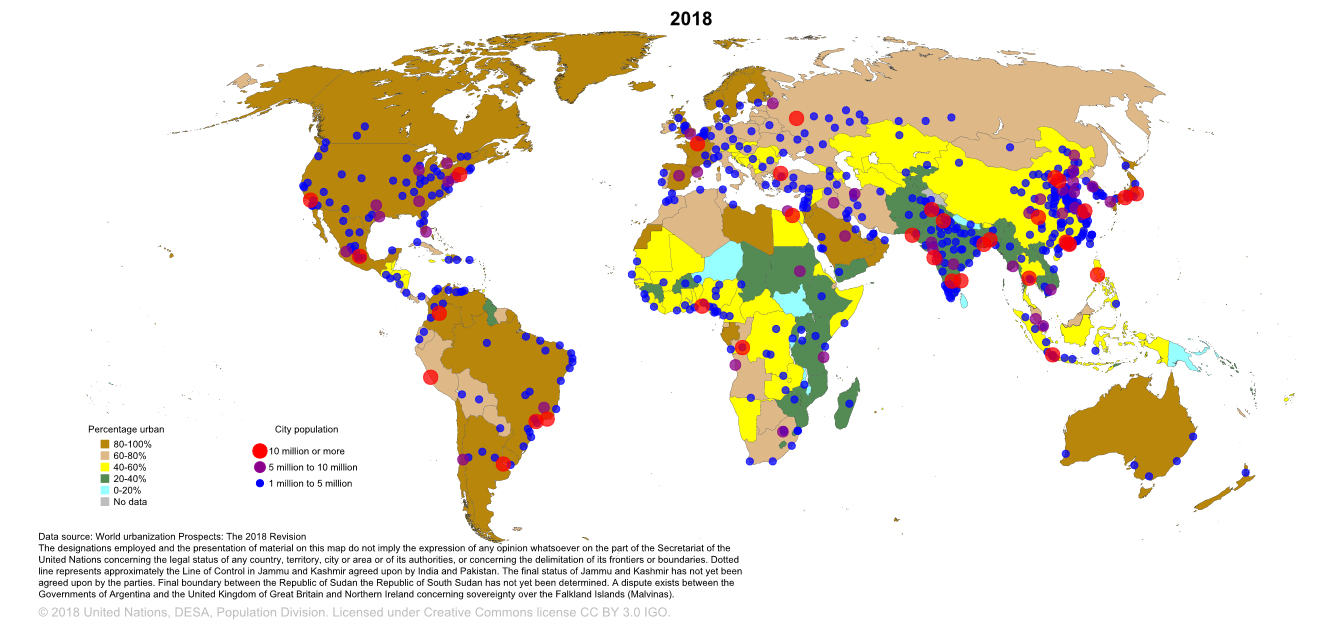
\includegraphics[width=20cm]{image_folder/CityPop_Urban.png}
\caption{Urbanisierung der Welt}
\label{figUrban}
\end{figure}

In der obigen Abbildung erkennt man, dass Nord- und Südamerika sowie Europa deutlich verstädtert sind, wohingegen viele Regionen in Afrika und Asien mehr ländliche Gebiete beinhalten. Wie gut wiederum die Lebensmittelversorgung und Infrastruktur in Megastädten ist, hängt von Megastadt zu Megastadt ab. Die Abbildung \ref{figUrbanRf} zeigt eine gute Übersicht der unterschiedlichen Verhältnisse. In dieser Forschungsarbeit der Stadtbegriff im Bezug zu ihrer fähigen Lebensmittelversorgung und Nachhaltigkeit betrachtet.


\begin{figure}[h]
\centering
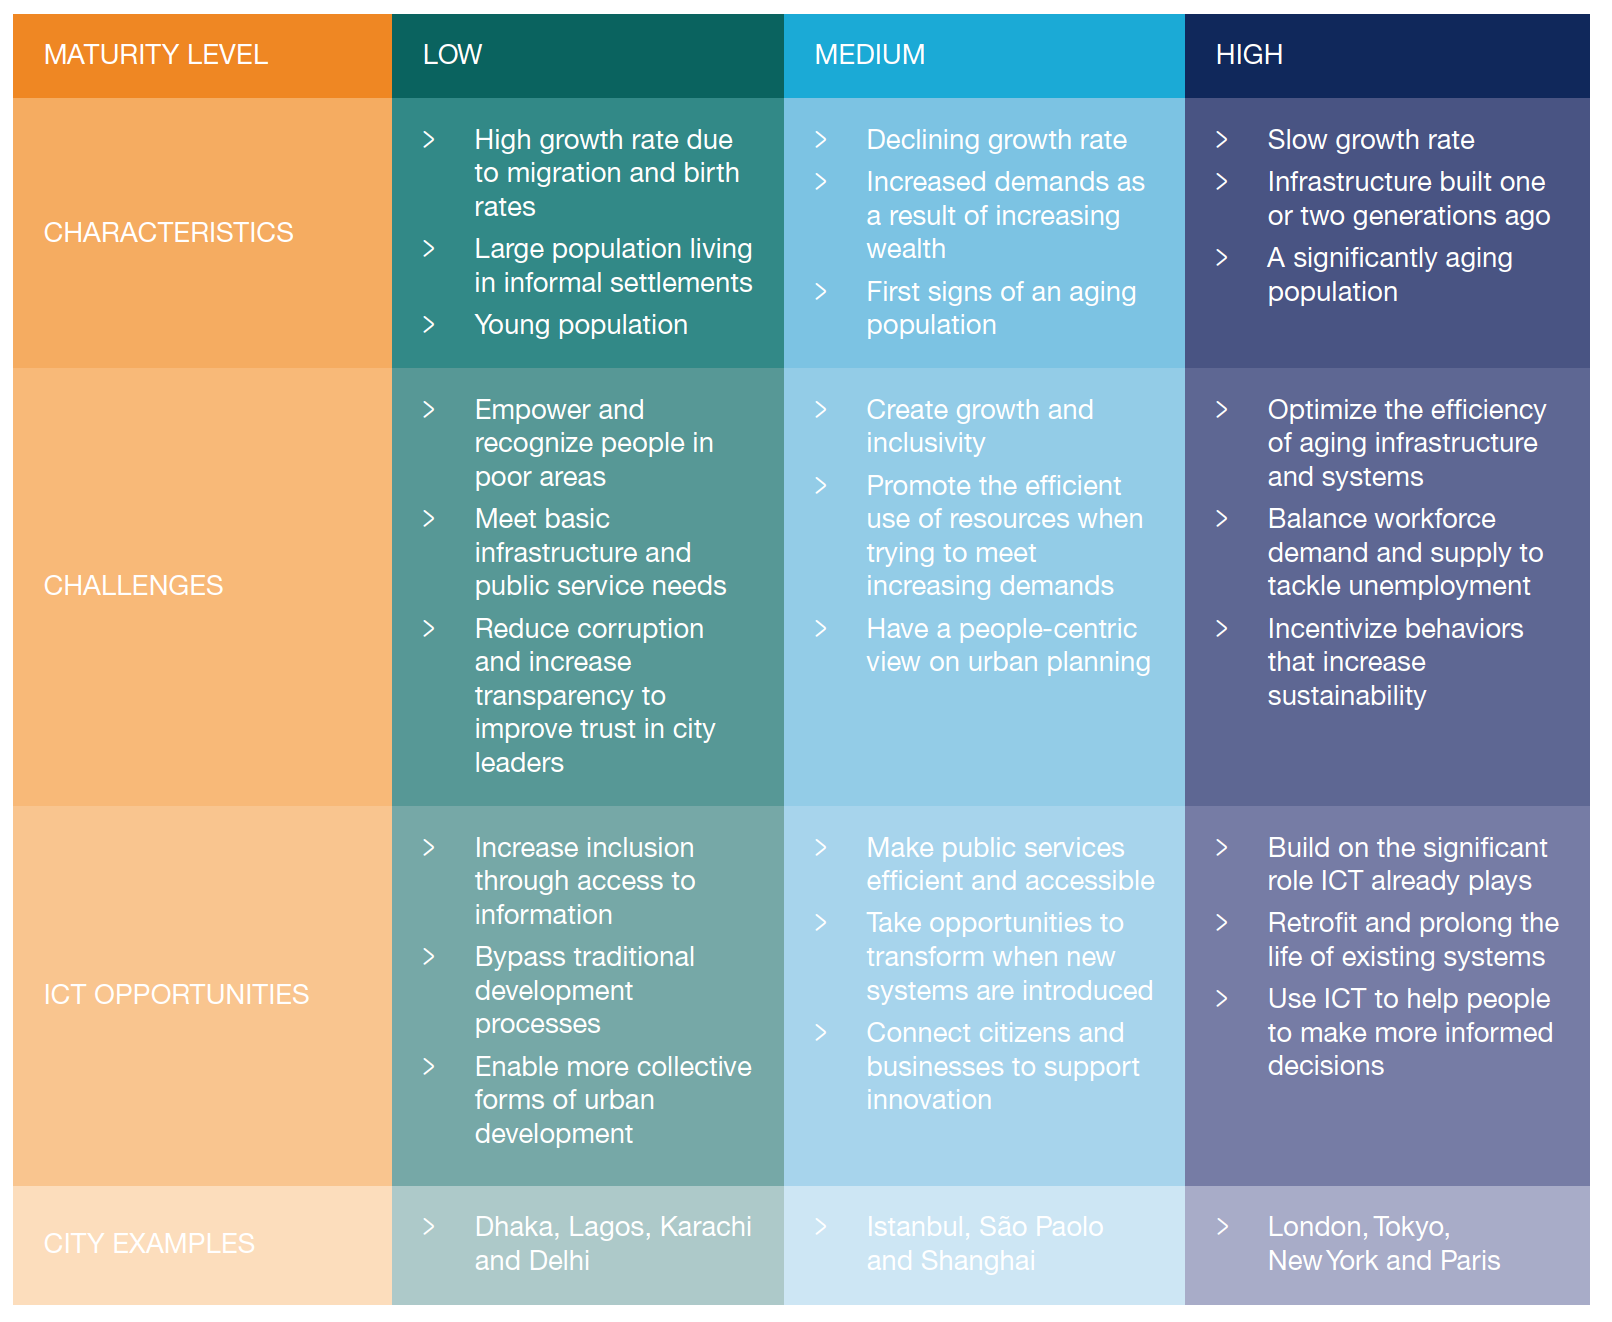
\includegraphics[width=10cm]{image_folder/urban_reifegrad.png}
\caption{Reifegrad von Megastädten}
\label{figUrbanRf}
\end{figure}

\subsubsection{Stadtökosysteme}
Stadtökosysteme sind Ökosysteme, die von Menschen erzeugt und beeinflusst werden. Wesentliche Merkmale eines Stadtökosystems sind der hohe Anteil an bebauter und versiegelter Fläche und eine hohe Bevölkerungsdichte. Genauer gesagt führt diese hohe Dichte an verschiedenen Landnutzungen dazu, dass natürlichen Ressourcen wie Wasser, Luft, Boden und Biodiversität extrem beansprucht werden. Desweiteren lässt sich über Stadtökosysteme sagen, dass ihr Erhalt von der externen Einfuhr an Lebensmitteln und Ressourcen abhängig ist  \cite[S.61]{Breuste2016Stadtokosysteme}.


\subsection{Nachhaltigkeit}

Der Begriff Nachhaltigkeit ansich ist ein vielschichtiger Begriff. Er findet Verwendung in der Wirtschaft, Ökonomie, Ethik und Ökologie. So kann Nachhaltigkeit als Art und Weise des Wirtschaftens bezeichnet, „bei welcher derzeitige Bedürfnisse befriedigt werden, ohne zukünftigen Generationen die Lebensgrundlagen zu entziehen (Sustainable Development). \cite{DefinitionWirtschaftslexikonb}. Ebenso kann der Begriff als Brücke zwischen ökologischen und ökonomischen Interessen gesehen werden. Seinen Ursprung hat das Prinzip der Nachhaltigkeit in der Forstwirtschaft des 18. Jahrhunderts. Nach einer Übernutzung der Wälder und daraus resultierend knapper werdenden Holzbeständen, wurde mit Nachhaltigkeit ein Bewirtschaftungsprinzip gefordert, bei dem regenerativ gearbeitet werden sollte, das heißt “nicht mehr Holz geschlagen werden als nachwächst.“\cite{NachhaltigeBrockhaus.de}
Ab dem 19. Jahrhundert wurde zu dieser rein ressourcenökonomischen Betrachtungsweise von Nachhaltigkeit eine Umfassendere hinzugefügt, die sämtliche Funktionen des Waldes in Betracht zieht.






Der Begriff Nachhaltigkeit kann in stark und schwach eingeteilt werden.\cite{Nachhaltigkeit}


\begin{itemize}
\item starke Nachhaltigkeit: Erhaltung der natürlichen Ressourcen steht im Vordergrund.Es beruht auf der Annahme, dass Naturgut nicht durch andere Kapitalformen ersetzt werden kann,
\item schwache Nachhaltigkeit beruht auf der Annahme das Kapital- oder Naturgut durch andere Kapitalformen erstz werden kann.
\end{itemize}
Konfliktpotenzial zwischen den Vertretern jeweiliger Positionen treten vor allem bei der Frage auf, "wie heute verursachte, aber zukünftig auftretende Umweltschäden beziehungsweise Ressourcenknappheiten zu bewerten sind.\cite{NachhaltigeBrockhaus.de}



\subsubsection{Nachhaltige Entwicklung}
 Dieser Begriff wurde von N. abgeleitet. In der internationaler Politik und bei gesellschaftlichen Bewegungen wird er als Leitbild eingesetzt. Ziel der Nachhaltigen Entwicklung ist eine dauerhalfte und gerechten Bewirtschaftung der Erde. \cite{NachhaltigeBrockhaus.de} In der Agrar- und Ernährungswirtschaft zielt der Begriff auf eine " dauerhafte Nutzung von Ressourcen bei gleichbleibender bzw. wachsender Effektivität". \cite{oppenhauser2010nachhaltigkeit} Im internationalen Sprachraum hat sich der Begriff Sustainable Development als Definition dieses Leitbild gefestigt.
 
 Konkrete Umsetzungsmethoden von Nachhaltiger Entwicklung stellen in Entwicklungsländern hauptsächlich Entwicklungsaspekte in den Vordergrund, in den industrialisierten Ländern geht es um den langfristigen Schutz und Erhalt der natürlichen Lebensgrundlage. 

\subsubsection{Konfliktpotenziale bei der Umsetzung von Nachhaltiger Entwicklung}

Die gerechte verteilung der endlichen ressorcen (global commons)

Das Rio-Abkommen aus dem Jahr 1992 wurde neben der Frage nach der Verantwortung für die Verursachung von Umweltproblemen die “Gerechtigkeitsfrage […] von zahlreichen Kommentatoren so beantwortet, dass im Prinzip jeder Mensch weltweit das gleiche Recht hat, die globalen Gemeinschaftsgüter in nachhaltiger Weise zu nutzen. Dieser Interpretation wird entgegengehalten, dass sie regional unterschiedliche Bedürftigkeiten und kulturelle Besonderheiten ignoriere.” cite{NachhaltigeBrockhaus.de}Ebenso besteht der "Einwand, dass neben den unterschiedlichen Bedürftigkeiten auch das unterschiedliche Leistungsvermögen berücksichtigt werden müsse. Demnach sei das zulässige Nutzungsniveau eines Staates nicht nach der Größe seiner Bevölkerung, sondern nach seinem Beitrag zur globalen Wertschöpfung zu bestimmen." \cite{NachhaltigeBrockhaus.de}

\begin{figure}[h]
\centering
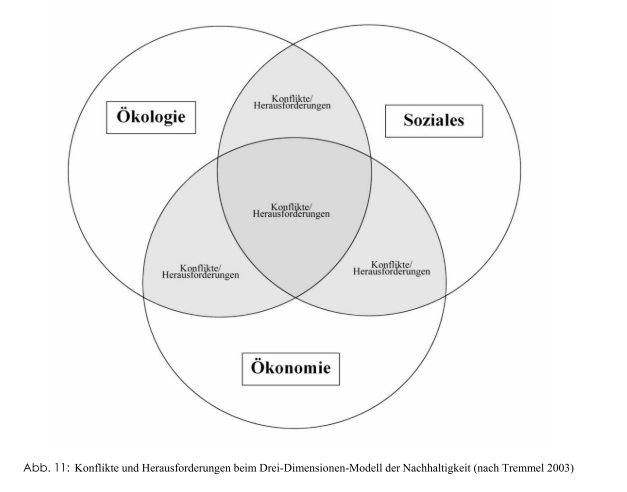
\includegraphics[width=10cm]{image_folder/dreidimensionenmodell_der_N.png}
\caption{3-dim-Modell}
\label{fig:3-dimensionen Modell}
\end{figure}

Konfliktpoltenzial besteht ebenfalls bei der Priorisierung von Lösungsvorschlägen. Eine Nachhaltige Lösung im sozialen Sinn kann auf Kosten von ökologischer Nachhaltigkeit gehen und umgekehrt. Genauso kann auch eine Win-Win Situation entstehen.

Länder des Südens stellen bislang die sozialen und ökonomischen Aspekte in den Vordergrund, Länder des Nordens wird dadurch die Hauptlast bei der Lösung der bestehenden Probleme im Ökologischen Bereich zugeschrieben. Die Länder des Nordens stellen ök. Apekt in den Vordergrund, nicht zuletzt weil sie es sich leisten können. SIe fordern gleichzeitig Lösungsinitative von Ländern des Südens.

\begin{figure}[h]
\centering
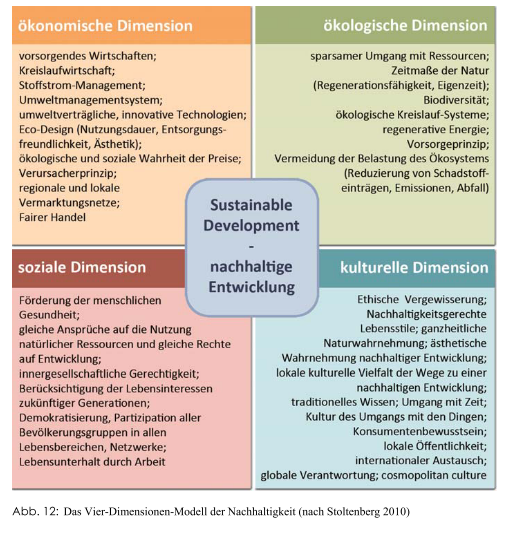
\includegraphics[width=6cm]{image_folder/vierdimensionenmodell_der_N.png}
\caption{4-dim-Modell}
\label{fig:4-dimensionen Modell}
\end{figure}

\subsubsection{Kritik am Begriff der nachhaltigen Entwicklung}(\cite{NachhaltigeBrockhaus.de})
Die übermäßige Verwendung des Begriff führt bei vielen Kritikern zu Misstrauen. Folgende Meinungen werden vertreten:

\begin{itemize}
\item Begriff sei überladen und als Sammelbegriff für alles Gute, was unerfüllbare Erwartungen wecke
\item Nachhaltige Entwicklung sei utopisch und eine Illusion
\item Beliebigkeit des Begriffs: “Unter der Flagge der nachhaltigen Entwicklung könne man trotzdem für komplett gegensätzliche Dinge eintreten.”
\item Meinung: Nachhaltigkeit sei inhaltslos und habe nur rhetorische FUnktionen, was die Leitbildfähigkeit des Begriffs außer Kraft setze
\end{itemize}

\subsubsection{Ökologische Nachhaltigkeit}
„Die ökologische Nachhaltigkeit bezieht sich allgemein auf das Überleben und den Gesundheitszustand von Ökosystemen.“ \cite{DefinitionWirtschaftslexikonc}  Sie bezeichnet einen weitsichtiger und rücksichtsvoller Umgang mit natürlichen Ressourcen. Sofern die ökologische Nachhaltigkeit vernachlässigt wird, kann dies dazu führen, dass bestimmte Ressourcen unbrauchbar oder unwiderruflich zerstört werden mit dem Ergebnis, dass auf diese Weise jegliche weitere Entwicklungen unmöglich werden. Laut Berding und Bukow in :Die kompakte Stadt der Zukunft Auf dem Weg zu einer inklusiven und nachhaltigen Stadtgesellschaft (s.95) \cite{BerdingWolf-DietrichBukowKarinCudakHrsgDieStadtgesellschaft} gewinnt das Thema Nachhaltigkeit für die Stadtentwicklung an Wichtigkeit. 



\subsubsection{Ökosystem}
Als Ökosystem bezeichnet man ein Wirkungsgefüge von Arten und ihrem Lebensraum. Es besteht aus Produzenten und Destruenten/Reduzenten. Dazwischen befindet sich eine Reihe an Konsumenten. -> Es entsteht eine Nahrungskette. Dieses Nebeneinander auf kleistem Raum aus Pflanzen und Tieren befindet sich in einem zyklischen Prozess. Je enger diese Nahrungskette ineinander verwoben sind und je Artenreicher das Wirkungsgefüge ist desto komplexer ist das Ökosystem.\cite{NachhaltigeBrockhaus.de} Die Agrarlandschaft kann als ein vom Menschen stark beeinflusstes und künstliches Ökosystem angesehen werden.
Ökosysteme sind offene Systeme, die einseitig von der Sonne Energie aufnehmen. Die Stoffkreisläufe inerhalb des Systems sind unter optimalen Umständen ausgeglichen. Es entsteht ein dynamisches Gleichgewicht.

Stabilität und Gefährdung: Komplexe Ökosysteme sind stabiler als einfache Ökosysteme, gleichzeitig, sind diese schwer oder unmöglich regenerierbar, während einfache Ökosysteme sich und ihr Gleichgewicht einfach widerherstellen können. Als Beispiel kann der Vergleich zwischen einfachem Ökosystem Nadelwald und komplexem Regenwald herangezogen werden.
Der Verlust oder die Veränderung einzelner Komponenten (Überdüngung, Wasserknappheit oder Bewässerung in Brachregionen) kann das eigene Gleichgewicht sowie das Gleichgewicht angrenzender Ökosysteme in Gefahr bringen. \cite{DefinitionWirtschaftslexikone}

\begin{figure}[htp]
\centering
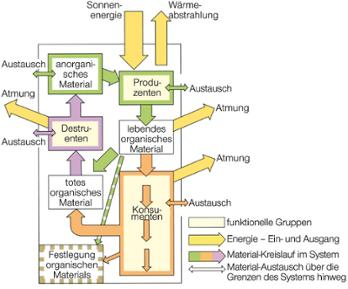
\includegraphics[width=5cm]{image_folder/oekosystemkreisslauf.png}
\caption{Ökosystemkreisslauf: Kreislauf: Verknüpfung von Konsumenten Destruenten und Produzenten}
\label{fig:Ökosystemkreisslauf}
\end{figure}
        
\subsubsection{Ökoeffizienz}
 Der World Business Council of Sustainable Development (WBCSD) hat " für Ökoeffizienz die folgenden Kriterien erstellt: die Bereitstellung wettbewerbsfähiger Produkte, die menschliche Bedürfnisse befriedigen, die Lebensqualität fördern und dabei die Umweltauswirkungen und Ressourcenintensität während des gesamten Produktlebens minimieren." \cite{OkoeffizienzBrockhaus.de}

Als Ökoeffizient werden Strategien und Konzepte bezeichnet, die sich dazu eignen nachhaltige Produktionsmethoden umzusetzen. Die Kriterien sind laut des World Business Council of Sustainable Development (WBCSD)– ein Zusammenschluss international tätiger Unternehmen, der das Ziel hat, Wirtschaftswachstum und Nachhaltigkeit in Einklang zu bringen Folgende:
\begin{itemize}
\item geringer Einsatz natürlicher Ressourcen
\item geringe Umweltbelastung
\item zu ersteren beiden im Vergleich hoher Ertrag
\end{itemize}

\begin{figure}[h]
\centering
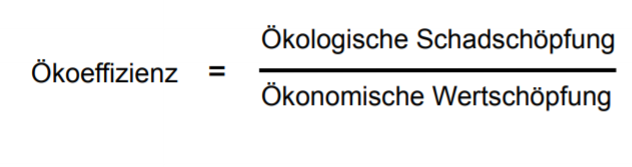
\includegraphics[width=5cm]{image_folder/oekoeffizienz.png}
\caption{Ökoeffizienzgleichung}
\label{fig:Ökoeffizienzgleichung}
\end{figure}\cite{Essel2010AnalyseFazit}


Ökoeffizienz kann u.a. erreicht werden durch:
\begin{itemize}
\item Minimierung des Material- und Energieverbrauchs pro Produktmenge,
\item Verwendung recyclingfähiger Materialien,
\item Einsatz erneuerbarer Ressourcen, Vermeidung des Einsatzes toxischer Substanzen,
\item Erhöhung der Lebensdauer beziehungsweise des Nutzens eines Produktes.
\end{itemize}

Methodische Ansätze zur Messung der Ökoeffizienz von Produkten sind:
\begin{itemize}
\item Stoffstrommanagement,
\item die Umweltbilanz
\item Ökoeffizienz-Analyse Bewertungsmethode der BASF." Sie entstand 1995 und bewertet die Wirtschaftlichkeit eines Produkts im Verhältnis zu der Umweltbelastung, die sie ausübt. Betrachtet wird der gesamte Lebensweg des Produkts beginnend bei der Rohstoffgewinnung über die Herstellung und Verwendung bis zur Entsorgung.
\end{itemize}
\cite{DefinitionWirtschaftslexikonc} (Quelle des gesamten Abschnitts)

\subsubsection{Bewertung von Nachhaltigkeit}
Werkzeuge zur Bewertung von Nachhaltigkeit: (nach welchen kriterien kann nachhaltigkeit beurteilt werden? (schon bei def?)

\begin{itemize}
\itemÖkoeffizienz-Analyse Bewertung von Nachhaltigkeit mit der \itemÖkoeffizienz-Analyse und SEEBALANCE®
\item GEMIS-Projekte
\item IINAS: Entwicklung eines globalen Nachhaltigkeitsstandards zur Landnutzung (GLOBALANDS)
\item Nachhaltigkeitsstrategien
\end{itemize}

\subsubsection{ökologischer Fußabdruck}
"Die (Natur-)Fläche, die zur Aufrechterhaltung der Energie- und Materialflüsse einer Wirtschaftsein-heit wie z. B. einer Stadt benötigt wird, ist deren ökologischer Fußabdruck. Er ist ein Werkzeug zur Bilanzierung des menschlichen Naturverbrauchs und wird in globalen Hektaren angegeben (vgl. Wackernagel & Rees 1997, 23–25). „Der ökologische Fußabdruck misst so die‚ ökologische Tragfähigkeit’ einer Bevölkerung“ (Wackernagel & Rees 1997: 25)."(Zitaat ausGrundlagen einer nachhaltigen Entwicklung S.5)

\subsubsection{Nachhaltigkeitswissenschaften}
Allgemein lässt sich festhalten, dass die "Nachhaltigkeitsforschung [...] sich mit Problemen, die die langfristige Sicherung der gesellschaftlichen Entwick-lungsbedingungen gefährden" befasst. MichelsenGrundlagenEntwicklung \cite{Grundlagen einer nachhaltigen Entwicklung} S.126)
Ihre Anfänge hat die Nachhaltigkeitswissenschaft im Rahmen der Forschung zum Globalen Wandel in den späten 1980er Jahren. Die Autoren des Reports Grundlagen einer nachhaltigen Entwicklung vermuten, dass das aufkommende Problembewusstsein, nicht zuletzt beeinflusst von der Publikation „Die Grenzen des Wachstums“ (Meadows et al. 1972), eine verstärkte Forschung zu Fragen globaler Umweltprobleme hervorrief.
Drei internationale Großforschungsprogramme werden dabei insbesondere genannt: (1) das „International Geosphere-Biosphere Programme (IGBP)“, (2) das „World Climate Research Programme“ und (3) das
„International Research Programme on Biodiversity (DIVERSITAS)“.


\begin{figure}[htp]
\centering
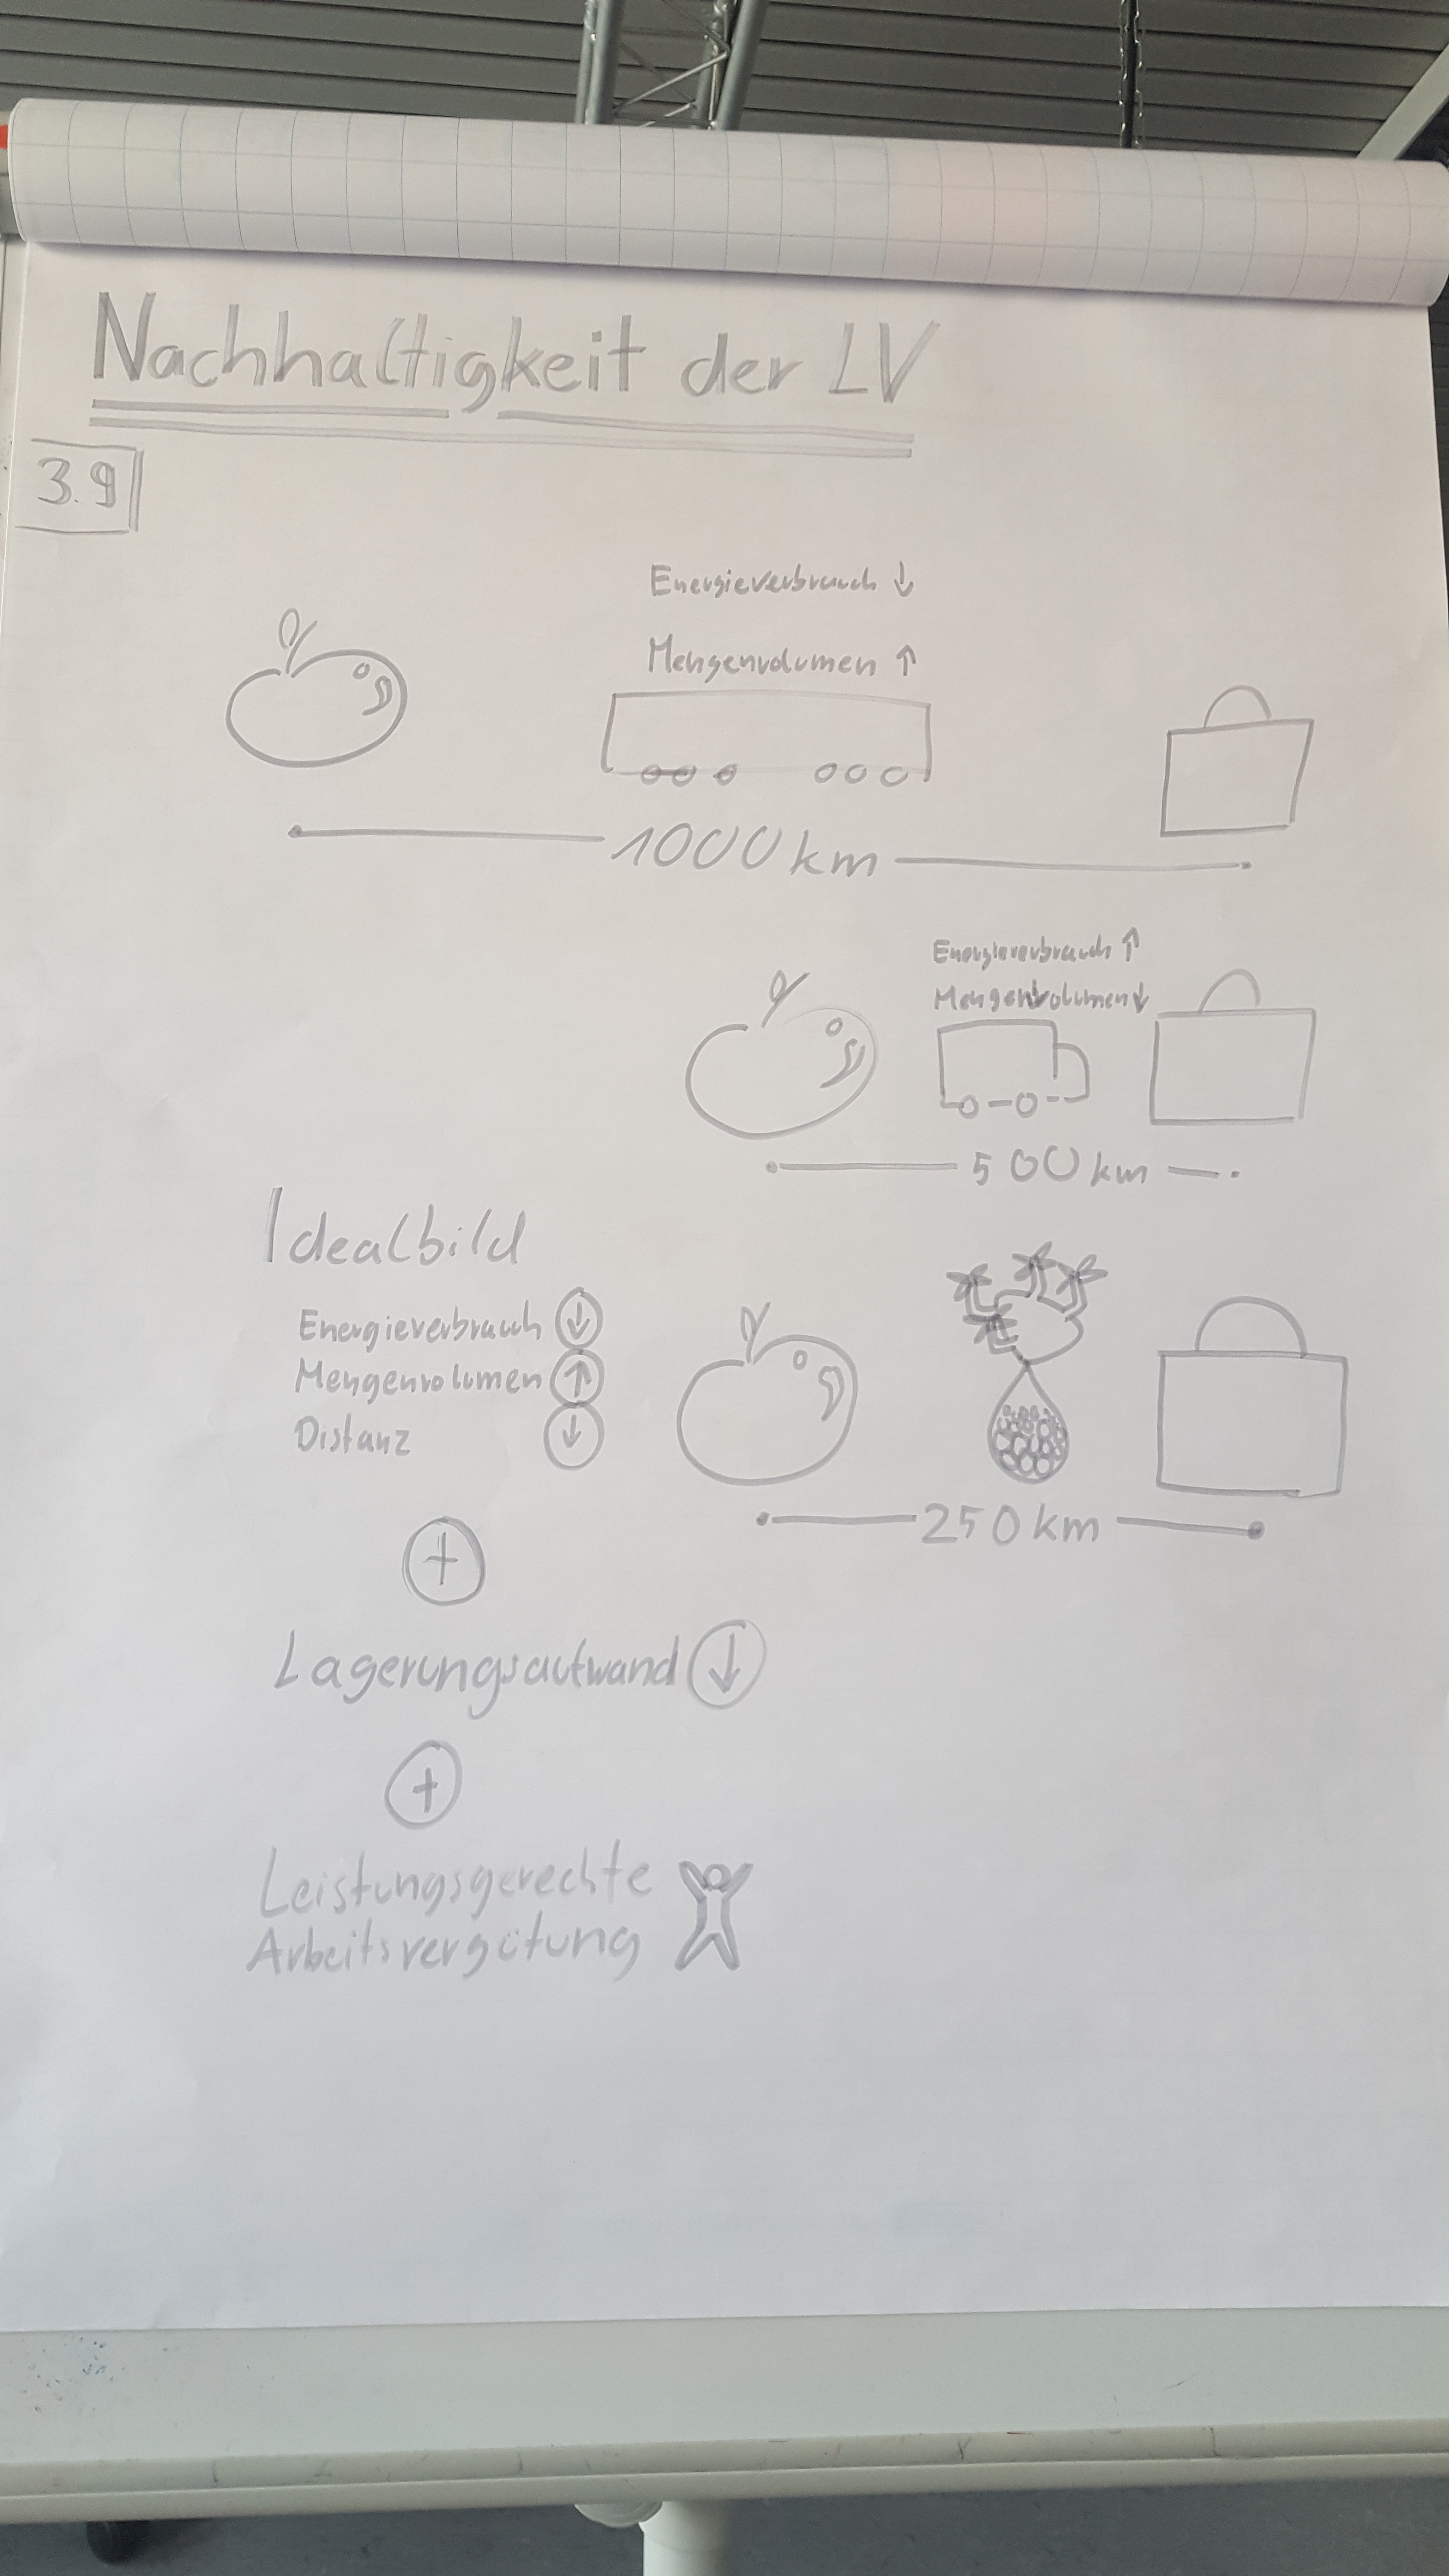
\includegraphics[width=5cm]{image_folder/skizze1.jpg}
\caption{Nachhaltigkeit der LV}
\label{fig:Skizze_Nachhaltigkeit}
\end{figure}

\section{Geschichte der Urbanisierung}
Wie Städte entstanden und sich bis heute ausbreiten hat viel damit zu tun wie sich die menschliche Versorgung von Nahrungsmitteln stetig weiterentwickelt hat. Elmquist, Redman, Barthel und Costanza beschreiben hierzu drei vergangene Lösungsansätze \cite{Elmqvist2013}. Der erste Ansatz war das Nomadentum. Menschen zogen von Gegend zu Gegend, um sich zu ernähren. Sie folgten Tierherden sowie klimatisch günstigeren Regionen, wo nahrhafte Rohstoffe zu finden waren. Der zweite Ansatz war die Domestizierung von Tieren und Pflanzen. Diese Form der Nahrungsmittelerzeugung erlaubte dauerhafte Sesshaftigkeit. Dadurch wurden kleine ländliche Gemeinden zur verbreitetesten Siedlungsform auf der Erde. Diese Gemeinden waren unabhängig und isoliert voneinander und zeichneten sich als besonders widerstandsfähig gegenüber klimatisch wechselnden Bedingungen aus. Die Folge dieses stabilen Lebensunterhaltes führte zu einer wachsenden Bevölkerung. Daraus entwickelte sich der dritte Lösungsansatz: Die „urbane Revolution“ %\cite{}. 
Dorfgemeinden wuchsen so sehr, dass die Menge an Menschen überschüssig zur nötigen Arbeit auf dem Acker war. Den Höhepunkt dieses Prozesses bildete 5500 v.C. die erste städtische Siedlung in Mesopotamien. Die daraus resultierenden Innovationen wie das Schreiben, Monumentalbauten oder spezialisiertes Handwerk zeigten klare Unterschiede zu vorherigen Siedlungsform. Desweiteren ergab sich daraus eine soziale Erneuerung, die charakteristisch für Städte war: Eine klassenstrukturierte Gesellschaft, eine formalisierte Rechtsgrundlage und eine territoriumsbasierte Regierung bildeten den funktionierenden Rahmen. Durch den stetigen Anstieg an Menschen war eine funktionierende Gesellschaftsform notwendig. Anders als die ländlichen Gemeinden zeichnete sich eine Stadt durch die äußerst divers und voneinander abhängig ist. 

\section{Vergangenheit der Urbanen Landwirtschaft}

Betrachtet man die Entwicklung und bisherige Ausgestaltung von Städten, kann man dahinter leicht ein bestimmtes System entdecken. Neben der eher durchdachten Verortung der Städte fand eine klare Differenzierung zum ländlichen Raum statt. Städte oder Siedlungen wurden
zwar wie bereits erwähnt in Gebieten gegründet, die Versorgung durch Trinkwasser und Nahrung sicherstellten, dennoch führte die urbane Verdichtung dazu dass Nahrungsmittel häufig aus dem Umland in die Städte befördert werden. Hierbei stellt die Megametropole New York ein Beispiel dar. Die Entwicklung der Stadt zeigt durch ihre verdichtete urbane Struktur eindeutig eine Tendenz, die die rurale Landwirtschaft oder ländliche Flächen "aussperrt" oder ihnen nur bedingt Platz bietet. Dennoch ist die Stadt durch die Nähe zum Atlantik und der ausgebauten Infrastruktur für eine Versorgung für Nahrungsmittel aus der ruralen Landwirtschaft gut gerüstet. Die Stadt selbst fungiert hierbei lediglich als Lebensraum und infrastrukturelle Anlaufstelle.

Dabei existieren bereits seit mehr als 100 Jahren Stadtpläne durch ambitionierte Stadtplaner die das "Ländliche" als solches für das Leben in einer
Stadt als essentiellen Bestandteil ansehen. Betrachtet man zum Beispiel einmal die Vision des britischen Sadtplaners Ebenezer Howard und seine Vision der Gartenstadt. Diese bildet noch heute ein Vorbild für moderne Stadtplaner. In seinem Buch "Garden Cities of Tomorrow" welches bereits 1898 verfasst wurde vertritt er das Konzept eines Zusammenspiels von ruraler Landwirtschaft und urbanen Gebieten. Er betont zudem dass es sich bei den
Gärten nicht nur um angelegte Ziergärten und Erholungsorte sowie Freizeitparks handelt sondern auch um "Freiräume", die Platz für den Anbau von
Nutzpflanzen und der Aufzucht von Nutztieren bieten sollen. Neben den frühen Gedanken an eine Landwirtschaft innerhalb städtischer Strukturen ist der Aspekt der Versorgung und Infrastruktur ebenfalls betrachtet worden.

\begin{figure}[htp]
\centering
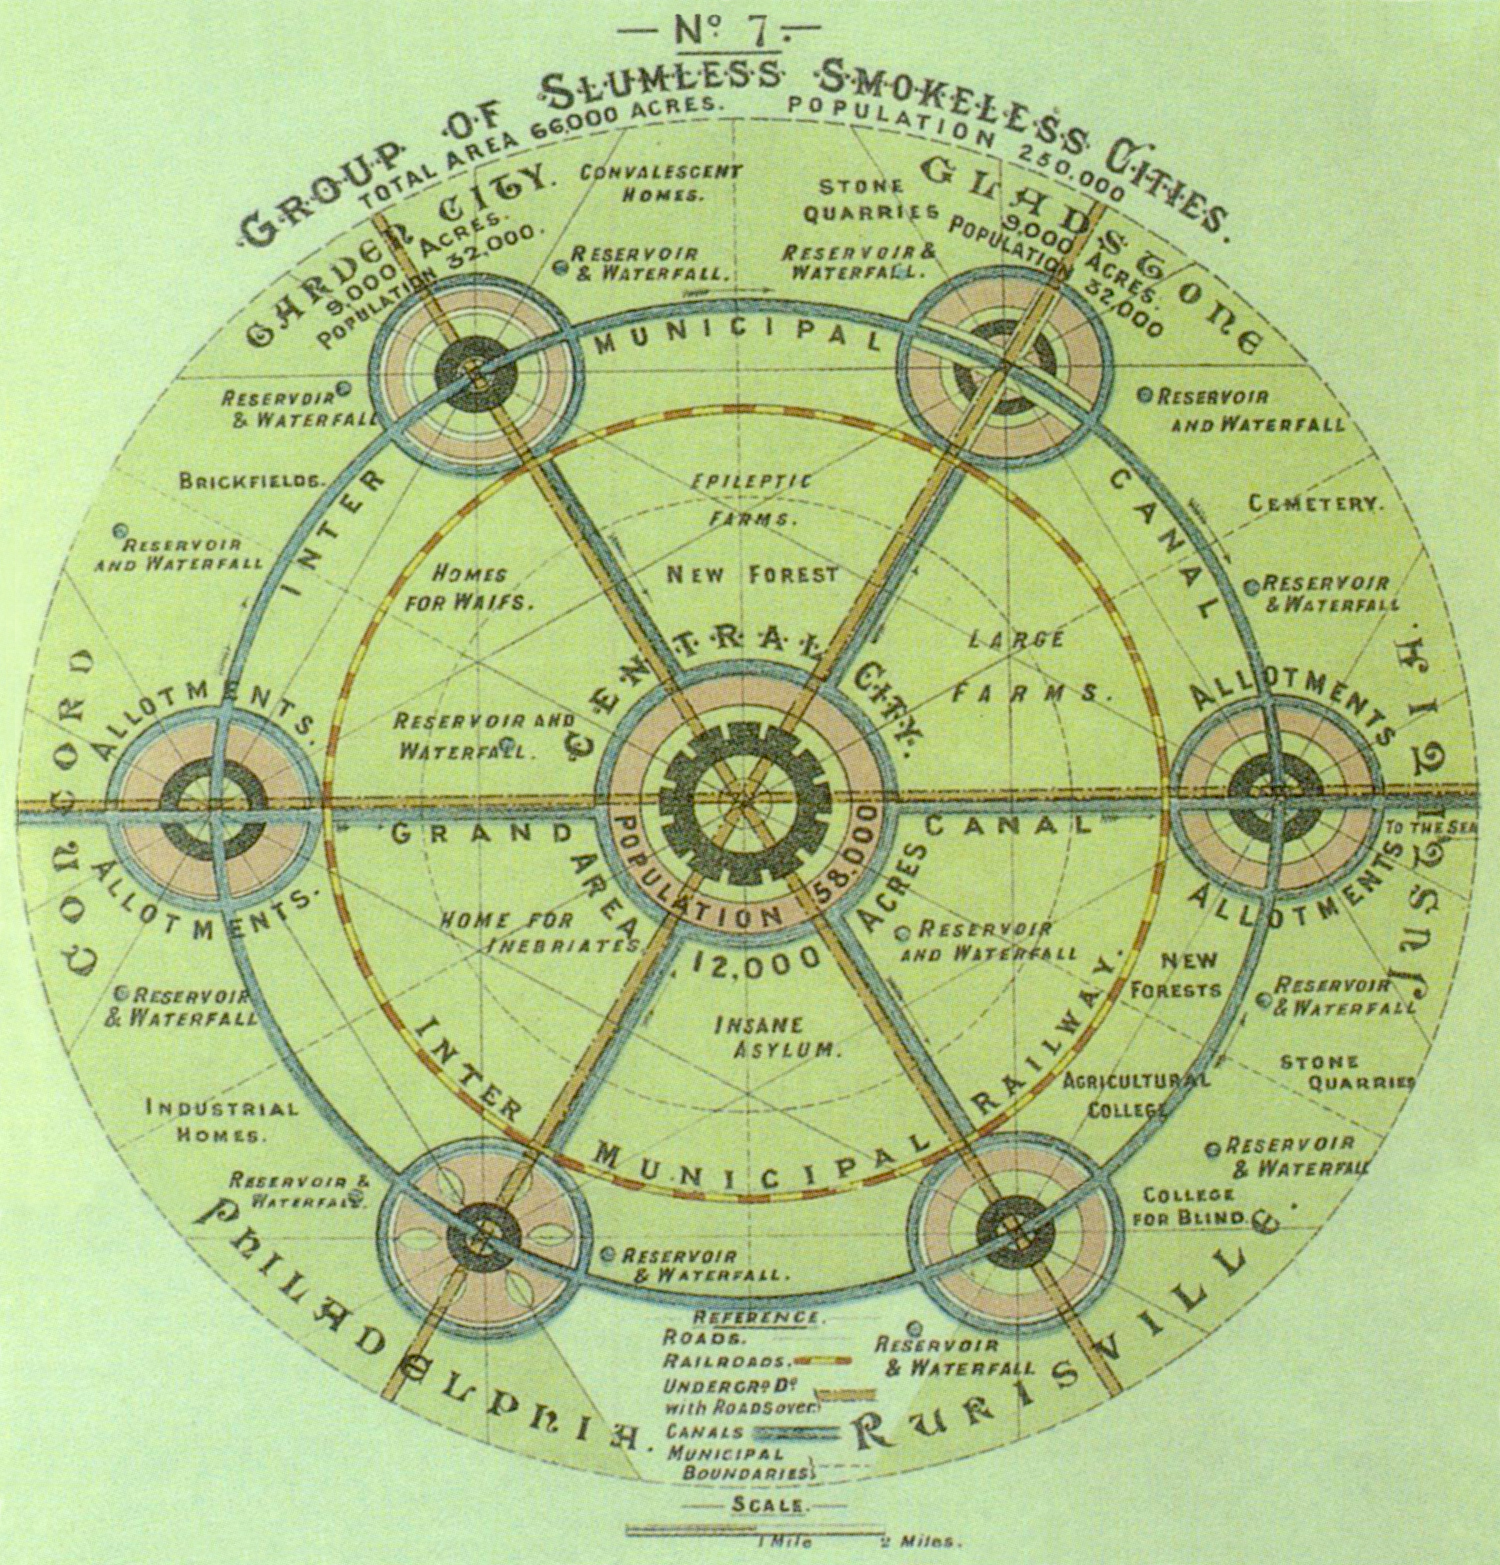
\includegraphics[width=10cm]{image_folder/GardenCityConcept_EbenezerHoward.jpg}
\caption{Konzept der Gartenstadt von Ebenezer Howard}
\label{fig:GardenCityConcept_EbenezerHoward}
\end{figure}

Interessant sind hier die "landwirtschaftlichen Gürtel" rings um die Städte und das Marktzentrum - den sogenanten "Crystal Palace" im Stadtzentrum.
Ein Ringförmiger Markt, der einem gläsernen Gewächshaus ähneln soll, das Waren aus der umliegenden Landwirtschaft direkt an den Verbraucher vertreiben kann. Generell bleibt festzuhalten, dass Howard bereits 1898 nicht nur ein Konzept zur Verankerung von Landwirtschaft innerhalb von urbanen Gebieten erdachte sondern auch Ideen entwickelte, wie die urbane Bevölkerung mit den Lebensmitteln versorgt werden kann.

Betrachtet man zum Beispiel Städte wie Boston, USA fällt auf, dass Grünflächen und Grünzüge nach dem Vorbild Howard´s zwar eine wichtige Rolle in der Stadtplanung spielen, diese Grünflächen aber meist als Parks und Freizeitanlagen angelegt wurden. Dies war lange das von der Allgemeinheit als "ländlich" verstandene Bild von Natur innerhalb einer Stadt.

Der urban landwirtschaftliche Aspekt wurde aber in den darauffolgenden Jahren durch nachfolgende Stadtplaner oft übergangen. Für den folgenden Stadtwachstum verkam die Urbane Landwirtschaft zur Ausgestaltung von mühevoll angelegten und vermeintlich natürlichen Ziergärten, die Grünflächen und Erholungsgebiete in die Städte bringen sollten. Aber wie kam es zu dieser gegensätzlichen Entwicklung?

In Deutschland zeigt die Sozialgeschichte das 1800 Großteile der Bevölkerung auf dem Land leben und aus der sogenannten unterbäuerlichen Schicht bestehen. Zu diesem Zeitpunkt gab es in Deutschland lediglich drei Großstädte. 1835 Endstand dann allmählich das Eisenbahnnetz welches maßgeblich zur Ausbreitung der Industrialisierung beitrug. Durch das Eisenbahnnetz konnten Arbeiter zu Ihren Arbeitsstätten pendeln, welche sich durch das wachsende Netz stärker ausbreiten konnten. Zudem konnten Güter verstärkt kostengünstig transportiert werden. Dies führte in den folgenden Jahren zum Wachstum der städtischen und ländlichen Gebiete und trug zudem zum Bevölkerungswachstum bei. 1850 bildete sich die industrielle Gesellschaft heraus und Deutschland umfasste bereits 35 Millionen Einwohner, welches damit als eines der größten Länder Europas zu dieser Zeit galt. Das enorme Städtewachstum wiederum ging auf die Binnenwanderungen, den Wachstum der Bevölkerung, Gebietserweiterungen und Eingemeindungen zurück. 1900 besaß Deutschland dann bereits 33 Städte mit mehr als 100 Tsd. Einwohnern. Der Ausbau des Schienennetzes ist dabei nicht der einzige Faktor oder gar der Grund der Industrialierung oder des Bevölkerungswachstums, dennoch trug es massiv zur Ausbreitung der Bevölkerung bei. Heinrich Heine einer der bedeutendsten deutschen Schriftsteller schrieb einmal „Welche Veränderungen müssen jetzt eintreten in unserer Anschauungsweise und in unsern Vorstellungen! Sogar die Elementarbegriffe von Zeit und Raum sind schwankend geworden. Durch die Eisenbahnen wird der Raum getötet, und es bleibt nur noch die Zeit übrig“. Dabei bot die Bahn natürlich nicht nur Vorteile. Sie trug maßgeblich zur Veränderung des Landschaftsbildes bei und brachte Rus und Lärm in die Landschaften und Städte. Durch wachsende Infrastrukturen und der Industrie aber verdichteten sich im laufe der 20. Jahrhunderts die urbanen Gebiete.

Lieberecht Migge schrieb 1926 in Hinblick auf diese Entwicklung "Das grüne Manifest" in dem er das "Leiden" der Städte zum Teil auf die Industrialisierung zurück führt. Er bezeichnet das "Land" (hier der ländlich rurale Freiraum) als Frischluftbehälter und als universale Erweiterungszone. Interessant ist hier auch dass er das "Land" nicht nur als physischen Freiraum sondern auch als Freiraum für den Geist des Menschen betrachtet in dem er seine Identität frei entfalten und entwickeln kann. Parolen ähnliche Leitsätze wie "Schafft Stadtland" oder "Die Städte sollten Ihr eigenes Land umarmen" implizieren die Grundidee des ruralen Raumes innerhalb der Stadtgebiete. "Man Pflanze!" heißt es weiter. Aber das Gepflanzte soll auch Mehrwert erfüllen, keine einfachen nach Blumenbeet anmutenden Grünflächen um der Optik willen, sondern Parkanlagen, Spielplätze und Bäder, die der Allgemeinheit einen Mehrwert bieten. Aber auch Gedanken zur Selbstversorgung kommen auf. So schreibt er Beispielsweise von Nutzgärten mit einer größe von 80qm pro Einwohner auf denen Nahrungsmittel für den Eigenbedarf angebaut werden sollten. Was sich zunächst nach einer Wunschvorstellung anhört, könnte in Ausnahmesituationen Leben retten. Nach dem zweiten Weltkrieg litten beispielsweise viele Stadtbewohner an Nahrungsmangel. In der Nachkriegszeit änderte sich daher der Blick auf Urbane Landwirtschaft massiv. In städtischen Hinterhöfen wurden zum Beispiel auch Kartoffeln und Rüben angebaut. Erholungsparks und Spielplätze wurden in Nutzgärten gewandelt da reine Grünplätze mehr und mehr als unwirtschaftlich betrachtet wurden. Migge war sich dessen bewusst und versuchte in seinem Manifesto eine Art Richtlinie für den Städtebau zu entwickelten. So verurteilt er auch den Wohnraum einzelner Menschen über deren Bedarf hinweg und fordert ein verstärtkes Bewusstsein für Müll und Nahrungsmittel. Die Städter sollten in einer Art Gleichgewicht mit dem Land leben das betont er wei folgt: "Die Stadt muss auch geben dem Land - will sie leben vom Land". Eine der wichtigsten Architektonischen Eigenschaften von Städten, das Bauen von Wohneinheiten übereinander, verurteilt er und bezeichnet das "übereinander" als die Wurzel allen übels. Dies ist zwar eine äußerst radikale Ansicht, repräsentiert aber den Wunsch nach freier Entfaltung und individualität des Wohnraumes. Er wünschte sich weiter ein neues Dasein im ländlich urbanen Raum welches durch harte Arbeit, Bescheidenheit und Naturverbundenheit geprägt sein sollte.

Zusammen mit Howard und Migge erdachten viele Gelehrten intelligente Stadtkonzepte so auch Ernst May der 1922/23 Trabantenstädte erdachte, die von "Kulturbändern" umgeben sein sollten, auf diesen dann eine intensive Landwirtschaft entstehen sollte. Gemüse und Kleinvieh von Kleinbauern sollte so herangezogen und -gezüchtet werden, welches dann als Nahrungsmittel für die Siedlungen gefördert werden sollte. Dieser Ansatz floss in den 1920er Jahren in den Städtebau mit ein und stärkte dabei das Kleingartenwesen.

Mitt der 1970er Jahre erreichte dann die Iddee der Community Gardens Europa. Hier nutzten fleißige Anwohner benachteiligter Viertel, beispielweise in New York, Brachflächen der Stadt und pflanzten Blumen, Gemüse und Kräuter an. Diese Bewegung erreichte Deutschland etwa 1990. Berlin gilt heute als eine der deutschen Hochburgen für Gemeinschaftsgärten. Zusammenfassend lässt sich sagen, dass urbane Landwirtschaft häufig als Rettungsring betrachtet wird. Das Bewusstsein für die vermeintlich lebensrettende Methode der Landwirtschaft scheint immer dann stark zu wachsen wenn es den Bewohnern urbaner Gebiete besonders schlecht ergeht. Dies wurde auch 2007 deutlich als schwere Waldbrände in Griechenland wüteten. Die Krise führte zu einem vermehrten Anbau von Nahrungsmitteln innerhalb der griechischen Städte und führte sogar zur Ausbeutung von städtisch landwirtschaftlichen Räumen durch Zivilisten. Seit 2012 wird die urbane Landwirtschaft von der Zivilgesellschaft oder den einzelnen Gemeinden verbreitet.

Ein weiteres Beispiel für den Antrieb von Urbaner Landwirtschaft in Kriesenzeiten lieferte Kuba in den 90er Jahren. Durch den Zusammenbruch der Sowjetunion kam es auf der Insel auch zum Zusammenbruch der dortigen Wirtschaft, da diese stark von der sowjetischen Ölversorgung abhing. Durch den fehlenden Rohstoff konnten beispielsweise keine Erntemaschinen betankt werden. Zudem mangelte es auch an Düngern und Pestiziden. Die Einwohner der Insel setzten immer stärker auf die urbanen Anbaumethoden. Heute gehört der Inselstaat zu den Ländern die große Fortschritte zur Bekämpfung von Hunger durch Urbane Landwirtschaft gemacht haben.

Detroit welche von einer starken Wirtschaft profitierte geriet vor Jahrzehnten in eine schwere Krise. Die einstige florierende Automobilbranche liegt brach. Dadurch zogen viele arbeitslose Einwohner aus der Stadt. Durch die ungenutzten urbanen Gebiete konnte aber in den darauffolgenden Jahren eine aufsteigende Landwirtschaft entstehen. Brachland und Dachterrassen wurden nun zu ca. 1200 fruchtbare Gärten verwandelt. „Nach einer Studie der Michigan State University könnte Detroit mit Stadtfarmen, Nachbarschaftsgärten und Gewächshäusern drei Viertel ihres Gemüses und vierzig Prozent ihres Obstes selbst produzieren.“ https://www.bzfe.de/inhalt/gemuese-statt-cadillac-urban-gardening-in-detroit-27424.html

Urbane Landwirtschaft heute

Die Urbane Landwirtschaft hat es mittlerweile immer öfter in die öffentlichen Medien geschafft. Durch die Ansätze des Guerilla Gardenings oder Skyfarmings erzeugt das Themenfeld auch größeres Interesse, beinhaltet aber auch Projekte und Ansätze ohne deutlichen Mehrwert. Dies bedeutet das manche Methoden der UL einen unauschreichend Nachhaltigen Aspekt bieten oder schlichtweg nicht wirtschaftlich arbeiten. Beispiele für UL folgen in Kapitel X. Es kommt hinzu dass die UL keine nennenswerte Rolle in der Ausbildung von Landwirtschaftsberufen spielt. Das Bewusstsein für die moderne Stadt ändert sich durch ambitionierte Architekten, Stadtplaner und Einwohner dennoch stetig und Brachflächen innerhalb von Städten werden nicht mehr nur einfach begrünt sondern nehmen auch einen immer größeren Platz in der Planung ein. 

"Man versucht die Landwirtschaft als Partner zu gewinnen, um die Freiflächen in der Stadtregion zu unterhalten und als öffentlichen Raum zu bespielen." Frank Lohrberg - Urban Gardening Christa Müller

\subsubsection{Heutige und zukünftige globale Landnutzung}


Das Umdenken der allgemeinen Gesellschaft fandt dennoch erst zunemend nach dem ersten Weltkrieg statt. Zuvor 



\newpage
\listoffigures
\printbibliography
\end{document}
